% TODO; wie darf ich einen Meromorphen verändern, (das P verändern) ohne das
% sich effektiv was ändert?
% TODO: \cM = \cM_K ... replace
%TODO: Dimension eines Meromorphen Zusammenhang

\chapter{Der Meromorphe Zusammenhang}
%Quelle ist \cite{sabbah_cimpa90}
\begin{comment}
\begin{itemize}
\item wofür sind die gut?
\item wieso kommt man ursprünglich dazu
\end{itemize}
\end{comment}

\begin{comment}
%\section{Lokalisierung eines $\C\{x\}$-Moduls}
%\begin{defn} \cite[Chap 4.1.]{sabbah_cimpa90}
%Sei $M$ ein $\C\{x\}$-Modul und $K=\C\{x\}[x^{-1}]$, dann ist die
%Lokalisierung
%\[ M[x^{-1}]:=M\otimes_{\C\{x\}}K \,. \]
%\end{defn}

\section{Lokalisierung eines (holonomen) $\cD$-Moduls}
Sei $\cM$ ein links $\cD$-Modul. Betrachte $\cM$ als $\C\{x\}$-Modul und
definiere darauf
\[ M[x^{-1}]:=M\otimes_{\C\{x\}}K \]
als die Lokalisierung von $\cM$.
\begin{prop} \cite[Prop 4.2.1.]{sabbah_cimpa90}
$\cM[x^{-1}]$ bekommt in natürlicher weiße eine $\cD$-Modul Struktur.
\end{prop}
\begin{proof} \cite[Prop 4.2.1.]{sabbah_cimpa90}
mit:
\[
\partial_x(m\otimes x^{-k})=((\partial_xm)\otimes x^{-k})-km\otimes x^{-k-1}
\]
\end{proof}
\end{comment}

\section{Meromorpher Zusammenhang (Definition)}

%Besser?
%Allgemeiner?
\begin{defn}[Meromorpher Zusammenhang] \label{def:merom-zush}
Ein \emph{Meromorpher Zusammenhang}
$(\cM_K,\partial)$ besteht aus folgenden Daten:
\begin{itemize}
\item $\cM_K$, ein endlich dimensionaler $K$-Vektor Raum
\item einer $\C$-linearen Abbildung $\partial:\cM_K\rightarrow \cM_K$,
genannt \emph{Derivation} oder \emph{Zusammenhang}, welche für alle $f\in K$
und $u\in \cM_K$ die
\emph{Leibnitzregel}
\begin{equation}\label{eq:Leibnitzregel}
\partial(fu)=f'u+f\partial u
\end{equation}
erfüllen soll.
\end{itemize}
%Falls $k=K=\C(\{x\})$ reden wir von einem \emph{(konvergentem) Meromorphen
%Zusammenhang} und falls $k=\hat K=\Cful$ reden wir von einem \emph{formalen
%Meromorphen Zusammenhang}.
%TODO: korrekte benennung?
\end{defn}

\begin{bem}
\begin{enumerate}
\item Später wird man auf die Angabe von $\partial$ verichten und einfach
$\cM_K$ als den Meromorphen Zusammenhang bezeichnen.
\item Wir betrachten hier Meromorphe Zusammenhänge an $x=0$ als
Singularität.
\end{enumerate}
\end{bem}

\begin{defn}
\cite[1.a]{sabbah_Fourier-local}
Sei $\phi\in\C(\!(u)\!)$.
Wir schreiben $\sE^\phi$ für den (formalen) Rang 1 Vektorraum $\C(\!(u)\!)$
ausgestattet mit dem Zusammenhang $\nabla=\partial_u+\partial_u\phi$, im
speziellen also $\nabla_{\partial_u}1=\partial_u1=\phi'$.\\
\begin{comment}
Also
\begin{align*}
\sE^\phi=\Cful & \overset{\partial_u}{\rightarrow} \Cful\\
1              & \mapsto \phi'(u)\\
f(u)           & \mapsto f'(u)+f(u)\phi'(u)\\
\end{align*}
\end{comment}
\end{defn}

\begin{bem}
\cite[1.a]{sabbah_Fourier-local}
Es gilt $\sE^\phi\cong\sE^\psi$ genau dann wenn $\phi\equiv\psi \mod \Cfu$.
%TODO: hier formal oder konvergent?
\end{bem}

\section{Eigenschaften}
%Hier nun einige Eigenschaften Meromorpher Zusammenhänge.
\begin{comment}
\cite[4.2]{sabbah_cimpa90}
Let $\cM$ be a left $\cD$-module. First we consider it only as a
$\C\{x\}$-module and let $\cM[x^{-1}]$ be the localized module.
\end{comment}

%TODO: reihenfolge bei sabbah anderst!!!
\begin{lem}[Lemma vom zyklischen Vektor]
\cite[Thm 4.3.3]{sabbah_cimpa90}
\cite[Satz 4.8]{ZulaBarbara}
Sei $\cM_K$ ein Meromorpher Zusammenhang. Es Existiert ein Element
$m\in\cM_K$ und eine ganze Zahl $d$ so dass
$m,\partial_tm,\dots,\partial_t^{d-1}m$ eine $K$-Basis von $\cM_K$ ist.
\end{lem}
\begin{proof}
\cite[Satz 4.8]{ZulaBarbara}
\end{proof}

\begin{thm}
\cite[Thm 4.3.2]{sabbah_cimpa90}
Ein Meromorpher Zusammenhang bestimmt ein $\cD_K$-Modul
und andersherum.
\end{thm}
\begin{proof}
\cite[Thm 4.3.2]{sabbah_cimpa90}
\end{proof}

\begin{lem}
\cite[Satz 4.12]{ZulaBarbara}
\cite[Thm 4.3.2]{sabbah_cimpa90}
Ist $\cM_K$ ein Meromorpher Zusammenhang, dann existiert ein $P\in\cD_K$ so
dass $\cM_K\cong\cD_K/\cD_K\cdot P$.
\end{lem}
\begin{proof}
\cite[Satz 4.12]{ZulaBarbara}
\end{proof}
\begin{comment}
\begin{rem}
\cite[Proof of Theorem 5.4.7]{sabbah_cimpa90}
\[
\dim_{\hat K}\cM_{\hat K} =\deg P \mbox{ wenn } \cM_{\hat K}=\cD/\cD\cdot P
\]
\end{rem}
\end{comment}

\begin{lem}
Sei $(\cM_K,\partial)$ ein gegebener Meromorpher Zusammenhang, und $\phi$ ein
Basisisomorphismus von $K^r$ nach $\cM_K$, also in der Situation
\begin{center}
\begin{tikzpicture} [scale=3.3, descr/.style={fill=white,inner sep=2.5pt} ]
\matrix (m) [
  matrix of math nodes
  , row sep=3em
  , column sep=3em
  %, text height=3em
  %, text depth=0.25em
]
{
  \cM_K & \cM_K \\
  K^r   & K^r \\
};
\path[->,font=\scriptsize,>=angle 90]
(m-1-1) edge node[above]{$\partial$} (m-1-2)
(m-2-1) edge node[above]{$\phi^{-1}\circ\partial\circ\phi$} (m-2-2)
;
%TODO: make this harpoon arrows
\path[->,font=\scriptsize,>=angle 90]
(m-2-1) edge node[descr]{$\cong$} node[right]{$\phi$} (m-1-1)
(m-2-2) edge node[descr]{$\cong$} node[left]{$\phi$} (m-1-2)
;

\path[>=stealth,|->]
;
\end{tikzpicture}
\end{center}
gilt: $(K^r,\phi^{-1}\circ\partial\circ\phi)$ ist ebenfalls ein Meromorpher Zusammenhang.
\end{lem}
\begin{proof}
TODO, (3. Treffen)
\end{proof}
\begin{comment} %Allgemeiner
\begin{lem}
Sei $(\cM_K,\partial)$ ein gegebener Meromorpher Zusammenhang, und
$\phi:\cM\rightarrow\cN$ ein Isomorphismus so ist
$(\cN,\phi^{-1}\circ\partial\circ\phi)$ ein zu $(\cM_K,\partial)$ isomorpher
Zusammenhang.
\begin{center}
\begin{tikzpicture} [scale=3.3, descr/.style={fill=white,inner sep=2.5pt} ]
\matrix (m) [
  matrix of math nodes
  , row sep=3em
  , column sep=3em
  %, text height=3em
  %, text depth=0.25em
]
{
  \cM_K & \cM_K \\
  \cN   & \cN \\
};
\path[->,font=\scriptsize,>=angle 90]
(m-1-1) edge node[above]{$\partial$} (m-1-2)
(m-2-1) edge node[above]{$\phi^{-1}\circ\partial\circ\phi$} (m-2-2)
;
%TODO: make this harpoon arrows
\path[->,font=\scriptsize,>=angle 90]
(m-2-1) edge node[descr]{$\cong$} node[right]{$\phi$} (m-1-1)
(m-2-2) edge node[descr]{$\cong$} node[left]{$\phi$} (m-1-2)
;

\path[>=stealth,|->]
;
\end{tikzpicture}
\end{center}
\end{lem}
\begin{proof}
TODO, (3. Treffen)
\end{proof}
\end{comment}

\begin{lem} Sei $\cM_K\cong K^r$ ein endlich dimensionaler $K$-Vektor Raum mit
$\partial_1$ und $\partial_2$ zwei darauf definierte Derivationen. So gilt,
die differenz zweier Derivationen ist $K$-linear.
\end{lem}
\begin{proof}
Seien $\partial_1$ und $\partial_2$ zwei Derivationen auf $\cM_K$.
Da $\partial_1$ und $\partial_2$ $\C$-linear, ist $\partial_1-\partial_2$
$\C$-linear, also muss nur noch gezeigt werden, dass
$(\partial_1-\partial_2)(fu)=f\cdot(\partial_1-\partial_2)(u)$ $\forall f\in
K$ und $u\in\cM_K$ gilt.\\
%TODO: wieso gilt das?
\begin{align*}
(\partial_1-\partial_2)(fu) &= \partial_1(fu)-\partial_2(fu)\\
&= f'u+f\partial_1u-f'u-f\partial_2u\\
&= \underset{=0}{\underbrace{f'u-f'u}}+f\cdot(\partial_1u-\partial_2u)\\
&= f\cdot(\partial_1-\partial_2)(u)\\
\end{align*}
\end{proof}
\begin{cor}
Es sei $(K^r,\partial)$ ein Meromorpher Zusammenhang.  So ist
$\frac{d}{dz}-\partial:K^r\rightarrow K^r$ $K$-linear, also es existiert eine
Matrix $A\in M(r\times r,K)$ mit $\frac{d}{dz}-\partial=A$, also ist
$\partial=\frac{d}{dz}-A$.
\end{cor}

%TODO: beobachtung...

%TODO: differenz ist linear

\begin{defn}[Transformationsformel]
In der Situation

\begin{center}
\begin{tikzpicture} [scale=3.3, descr/.style={fill=white,inner sep=2.5pt} ]
\matrix (m) [
  matrix of math nodes
  , row sep=3em
  , column sep=3em
  %, text height=3em
  %, text depth=0.25em
]
{
  K^r &   &   & K^r \\
      & M & M & \\
  K^r &   &   & K^r \\
};
\path[->,font=\scriptsize,>=angle 90]
(m-1-1) edge node[descr]{$\cong$} node[above]{$\phi$} (m-2-2)
(m-3-1) edge node[descr]{$\cong$} node[above]{$\psi$} (m-2-2)
(m-1-4) edge node[descr]{$\cong$} node[above]{$\phi$} (m-2-3)
(m-3-4) edge node[descr]{$\cong$} node[above]{$\psi$} (m-2-3)

(m-2-2) edge node[above]{$\partial$} (m-2-3)

(m-1-1) edge node[above]{$\frac{d}{dz}+A$} (m-1-4)
(m-3-1) edge node[above]{$\frac{d}{dz}+B$} (m-3-4)

(m-3-1) edge node[descr]{$\cong$} node[right]{$T$} (m-1-1)
(m-3-4) edge node[descr]{$\cong$} node[left]{$T$} (m-1-4)
;

\path[>=stealth,|->]
;
\end{tikzpicture}
\end{center}
mit $\phi,\psi$ und $T$ $K$-Linear und $\partial,(\frac{d}{dz}+A)$ und
$(\frac{d}{dz}+B)$ $\C$-Linear, gilt:\\
Der Merom. Zush. $\frac{d}{dz}+A$ auf $K^r$ wird durch Basiswechsel $T\in
GL(r,K)$ zu
\[
\frac{d}{dz}+(T^{-1}\cdot T'+T^{-1}AT) = \frac{d}{dz}+B
\]
\end{defn}
\begin{defn}[Differenziell Äquivalent]
Man nennt $A$ und $B$ \emph{differenziell Äquivalent} ($A\sim B$) genau
dann, wenn es ein $T\in
GL(r,K)$ gibt, mit $B=T^{-1}\cdot T'+T^{-1}AT$.
\end{defn}

\begin{comment}
$1=TT^{-1}$ $\rightsquigarrow$ $T'T^{-1}+T(T^{-1})'=0$\\
$1=T^{-1}T$ $\rightsquigarrow$ $(T^{-1})'T+T^{-1}T'=0$
\end{comment}

\section{Newton Polygon} % ist dies eine Invariante??
% gestohlen aus der ZulaBarbara Seite 46
\begin{comment}
Quelle: sabba?
\end{comment}
Jedes $P\in \cD$ lässt sich eindeutig als
\[ P=\sum^{n}_{k=0}{\sum^{\infty}_{l=-N}{\alpha_{kl}t^l\partial_t^k}} \]
mit $\alpha_{kl}\in\C$ schreiben. Betrachte das zu $P$ dazugehörige
\[ H(P):=\underset{k,l\mbox{ mit }\alpha_{kl}\neq0}{\bigcup}\Big( (k,l-k) +
\R_{\leq 0}\times \R_{\geq 0} \Big) \subset \R^2 \,. \]
\begin{comment}
Bei Sabbah: $H\subset \N\times\Z$ und dann konvexe Hülle davon in $\R^2$
\end{comment}

\begin{defn} % aus der zula
Das Randpolygon von $\conv(H(P))$ heißt das \emph{Newton Polygon} von $P$ und
wird geschrieben als $N(P)$.
\end{defn}

\begin{defn} % aus der zula
Die Menge $\slopes(P)$ sind die nicht-vertikalen Steigungen von $N(P)$, die
sich echt rechts von $\{0\}\times\R$ befinden.\\ % der $y$-Achse
%TODO: bessere formulierung
\begin{itemize}
\item P heißt \emph{regulär singulär} $:\Leftrightarrow$
$\slopes(P)=\{0\}$, sonst \emph{irregulär singulär}.
\item Schreibe $\cP(\cM_K)$ für die Menge der zu $\cM_K$ gehörigen slopes
%TODO: wie sind die genau definiert? invariant?
\item Ein meromorpher Zusammenhang $\cM_K$ heißt regulär singulär, falls es
ein regulär singuläres $P$ gibt, mit $\cM_K\cong\cD/\cD\cdot P$
\end{itemize}
\end{defn}

\begin{exmp} \label{exmp:Newton-Polygon}
\begin{enumerate}
\item Ein besonders einfaches Beispiel ist 
$P_1=t^{\textcolor{red}1}\partial_t^{\textcolor{blue}2}$.  Es ist leicht
abzulesen, dass
\begin{align*}
\textcolor{blue}k &= \textcolor{blue}2 & 
\textcolor{red}l  &= \textcolor{red}1
\end{align*}
so dass
\[
H(P_1)=\Big( (\textcolor{blue}{2},\textcolor{red}{1}-\textcolor{blue}{2}) +
\R_{\leq 0}\times \R_{\geq 0} \Big) =\{(u,v)\in\R^2|u\leq 2, v\geq -1\} \,.
\]
In Abbildung \ref{fig:Newton-Polygon1} ist $H(P_1)$ (blau) sowie das Newton
Polygon eingezeichnet. Offensichtlich ist $\slopes(P_1)=\{0\}$ und damit ist
$P_1$ regulär singulär.
\item \cite[Bsp 5.3. 2.]{ZulaBarbara}
Sei $P_2=t^4(t+1)\partial_t^4+t\partial_t^2+\frac{1}{t}\partial_t+1$ so kann
man daraus das entsprechende Newton Polygon konstruieren.
Das Newton Polygon wurde in Abbildung \ref{fig:Newton-Polygon2} visualisiert.
\end{enumerate}
\end{exmp}
\begin{figure}[H]
%TODO: nummer aus der referenz ist falsch
\label{fig:Newton-Polygon}
\caption{Zu Beispiel \ref{exmp:Newton-Polygon}}
\centering
%\caption{Newton Polygon zu $P$ und $\rho^+P$}
\fbox{
  \subfloat[Newton Polygon zu $P_1$]{
    \label{fig:Newton-Polygon1}
    \begin{tikzpicture}
    \def\myPoints{{(2,-1)}}
    \def\myPath{(-.5,-1) -- (2,-1) -- (2,2)}
    \myNewtonPlot{\myPoints}{\myPath}{2}{-2}{2}{$N(P_1)$}
    \end{tikzpicture}
  }
  \quad
  \subfloat[Newton Polygon zu $P_2$]{
    \label{fig:Newton-Polygon2}
    \begin{tikzpicture} %[scale=1.5]
    \def\myPoints{{(0,0)}, {(1,-2)}, {(2,-1)}, {(4,0)}}
    \def\myPath{(-.5,-2) -- (1,-2) -- (4,0) -- (4,2)}
    \myNewtonPlot{\myPoints}{\myPath}{4}{-2}{2}{$N(P_2)$}
    \end{tikzpicture}
  }
}
\end{figure}

\begin{lem}
%TOTO: sabbah redet hier schon immer von \hat K, ist das nötig?
\cite[5.1]{sabbah_cimpa90} %TODO: genauer
\begin{enumerate}
\item $\cP(\cM_K)$ ist nicht Leer, wenn $\cM_K\neq\{0\}$
\item Wenn man eine exacte Sequenz
$0\rightarrow{\cM'}_K\rightarrow{\cM}_K\rightarrow{\cM''}_K\rightarrow0$
hat, so gilt $\cP(\cM_K)=\cP({\cM'}_K)\cup\cP({\cM''}_K)$.
% es gibt noch 2 weitere punkte
\end{enumerate}
\end{lem}

\section{Formale Meromorphe Zusammenhänge}
%
Definiere $ \hat\cD[x^{-1}]=\cD_\Cfx[x^{-1}]=\hat K<\partial_x>=:\cD_{\hat K} $
wobei $\hat K=\Cfu[x^{-1}]$.
\begin{comment}
bei ZulaBarbara ist $\hat \cD_{\hat K}=\Cful<\partial_u>$ hier $=\cD_{\hat K}$
\end{comment}
\begin{defn}[Formaler Meromorpher Zusammenhang]
Ein \emph{formaler Meromorpher Zusammenhang}
$(\cM_{\hat K},\partial)$ besteht, analog wie in Definition
\ref{def:merom-zush}, aus folgenden Daten:
\begin{itemize}
\item $\cM_{\hat K}$, ein endlich dimensionaler $\hat K$-Vektor Raum
\item einer $\C$-linearen Derivation $\partial:\cM_{\hat K}\rightarrow
\cM_{\hat K}$, welche die \emph{Leibnitzregel} (\ref{eq:Leibnitzregel})
erfüllen soll.
\end{itemize}
\end{defn}
\begin{bem}
Alle bisher getroffene Aussagen stimmen auch für formale Meromorphe
Zusammenhänge. Im besonderen existiert für jedes $\cM_{\hat K}$ ein ein $P\in
\cD_{\hat K}$ mit $\cM_{\hat K}=\cD_{\hat K}/\cD_{\hat K}\cdot P$.
\end{bem}

%TODO: titel: Operations on vector spaces with connection
%TODO: verzweigung statt pull-back?
\section{pull-back und push-forward}
%QUELLE: hottaetal.pdf Seite 21
\begin{comment}
\cite[1.3]{hotta2007d}
\end{comment}

Nach \cite[1.a]{sabbah_Fourier-local}. Sei $(\rho:\C\rightarrow \C , u\mapsto
t:=\rho(u))\in u\Cfu$ mit Bewertung $p\geq1$ und sei $\cM$ ein endlich
dimensionaler $\C(\!(t)\!)$ Vektorraum ausgestattet mit einem Zusammenhang
$\nabla$.
\begin{defn}[pull-back] \label{defn:pull-back}
\cite[1.a]{sabbah_Fourier-local}
Der \emph{pull-back (Inverses Bild)} $\rho^{+}\cM$ ist der Vektorraum
$\rho^{*}\cM=\C(\!(u)\!)\otimes_{\C(\!(t)\!)}\cM$ mit dem \emph{pull-back
Zusammenhang} $\rho^*\nabla$ definiert durch 
\begin{equation} \label{eq:pull-back-zusammenhang}
\partial_u(1\otimes m):=\rho'(u)\otimes\partial_tm \,.
\end{equation}
\end{defn}
%
\begin{lem} \label{lem:pull-back-hilfslemma1}
\def\myT{\cD_{\Cftl}}
\def\myU{\cD_{\Cful}}
Es gilt $\rho^*\myT=\Cful\otimes_{\Cftl}\myT \cong \myU$ mittels
\begin{center}
\begin{tikzpicture} [scale=3.3, descr/.style={fill=white,inner sep=2.5pt} ]
\matrix (m) [
  matrix of math nodes
  %, row sep=1.5em
  , column sep=3em
  %, text height=3em
  %, text depth=0.25em
]{
\Phi:\Cful\otimes_{\Cftl}\myT & \myU \\
%1\otimes m(t,\partial_t) & m(\rho(u),\rho'(u)^{-1}\partial_u) \\
f(u)\otimes m(t,\partial_t) & f(u)m(\rho(u),\rho'(u)^{-1}\partial_u) \\
};
%TODO: Pfeile
\path[->,font=\scriptsize,>=angle 90]
(m-1-1) edge node[above]{$\cong$} (m-1-2)
;
\path[|->,font=\scriptsize,>=angle 90]
(m-2-1) edge (m-2-2)
%(m-3-1) edge (m-3-2)
;
\end{tikzpicture}
\end{center}
\end{lem}
\begin{proof}
\end{proof}
\begin{bem}
Das soeben, in Lemma \ref{lem:pull-back-hilfslemma1}, definierte $\Phi$ erfüllt
für $1\otimes m$
\begin{align*}
\partial_u(1\otimes m) &\overset{\mbox{def}}{=} \rho'(u)\otimes\partial_t m \\
&\overset{\Phi}{\mapsto} \underset{=1}{\underbrace{\rho'(u)\rho'(u)^{-1}}}
  \partial_u m(\rho(u),\rho'(u)^{-1}\partial_u) \\
&= \partial_u m(\rho(u),\rho'(u)^{-1}\partial_u)\\
\end{align*}
und somit (\ref{eq:pull-back-zusammenhang}) wie gewollt.
\end{bem}
%
\begin{lem} \label{lem:pull-back-hilfslemma2}
\def\myT{\cD_{\Cftl}}
\def\myU{\cD_{\Cful}}
In der Situation
\begin{center}
\begin{tikzpicture} [scale=3.3, descr/.style={fill=white,inner sep=2.5pt} ]
\matrix (m) [
  matrix of math nodes
  , row sep=2.5em
  , column sep=5em
  %, text height=3em
  %, text depth=0.25em
]{
\Cful\otimes_{\Cftl}\myT & \Cful\otimes_{\Cftl}\myT \\
\myU & \myU \\
};
%TODO: Pfeile
%\path (m-1-1) edge[white] node{$\%$} (m-2-2);
\path[->,font=\scriptsize,>=angle 90]
(m-1-1) edge node[above]{$\id\otimes\_\!\cdot\! P(t,\partial_t)$} (m-1-2)
(m-1-1) edge node[left]{$\cong$} node[right]{$\Phi$} (m-2-1)
(m-1-2) edge node[left]{$\cong$} node[right]{$\Phi$} (m-2-2)
(m-2-1) edge node[above]{$\alpha$} (m-2-2)
;
\end{tikzpicture}
\end{center}
mit $\Phi$ wie in Lemma \ref{lem:pull-back-hilfslemma1}
macht $\alpha:=\_\!\cdot\! P(\rho(u),\rho'(u)^{-1}\partial_u)$ das Diagram
kommutativ.
\end{lem}
\begin{proof}
\end{proof}
%
\begin{lem}
Sie $Q\in\cD_\Cful\backslash \{0\}$.  Eine Abbildung der Form
$\cD_\Cful\overset{\_\cdot  Q}{\longrightarrow}\cD_\Cful$ 
%\begin{center}
%\begin{tikzpicture} [scale=3.3, descr/.style={fill=white,inner sep=2.5pt} ]
%\matrix (m) [
  %matrix of math nodes
  %, row sep=2.5em
  %, column sep=5em
  %%, text height=3em
  %%, text depth=0.25em
%]{
%\cD_\Cful & \cD_\Cful\\
%};
%%TODO: Pfeile
%%\path (m-1-1) edge[white] node{$\%$} (m-2-2);
%\path[->,font=\scriptsize,>=angle 90]
%(m-1-1) edge node[above]{$\_\cdot  Q$} (m-1-2)
%;
%\end{tikzpicture}
%\end{cen}
ist immer surjectiv.
\end{lem}
\begin{proof}
\begin{comment}
GEGENBEISPIEL:\\
$Q:=\partial_u$, $u\in\cD_\Cful$\\
suche ein $y$ so dass $y\partial_u=u$\\
\begin{align*}
\_\!\cdot\!  Q(y) &= u \\
y\partial_u       &= u \\
y\partial_u u     &= u u & \mbox{\cite[Chap. 4.]{sabbah_cimpa90} links
multiplikation mit $u$ ist nicht bijektiv} \\
y                 &= u^2 \\
\end{align*}
aber
\begin{align*}
u^2\partial_u &= u\cdot u\cdot \partial_u \\
  &=u\cdot (\partial_u\cdot u -1) \\
  &=u\cdot (1 -1) \\
  &=0 \\
\end{align*}
\end{comment}
\end{proof}
%
\begin{lem} \label{lem:pull-back-hilfslemma3}
%Wie erhält man den pull-back Zusammenhang bzw. wie ist er berechenbar? 
In der Situation von Lemma \ref{defn:pull-back}, mit
$\cM=\cD_{\Cftl}/\cD_{\Cftl}\cdot P(t,\partial_t)$ für ein
$P(t,\partial_t)\in\cD_{\Cftl}$, gilt
\[\rho^*\cM\cong \cD_{\Cful}\Big/\cD_{\Cful}\cdot
  P(\rho(u),\rho'(u)^{-1}\partial_u) \]
also wird der Übergang beschrieben durch
\begin{align*}
t          &\rightarrow \rho(t) \\
\partial_t &\rightarrow \rho'(t)^{-1}\partial_u \\
\end{align*}
\end{lem}
\begin{proof}
%TODO: warum hier alles Lokalisiert?
\def\myT{\cD_{\Cftl}}
\def\myU{\cD_{\Cful}}
Sei
$P\in\cD_\Cftl$ und $\cM:=\myT/\myT\cdot P$. Es ist
\begin{center}
  \begin{tikzpicture} [scale=3.3, descr/.style={fill=white,inner sep=2.5pt} ]
  \matrix (m) [
    matrix of math nodes
    %, row sep=1.5em
    , column sep=2.7em
    %, text height=3em
    %, text depth=0.25em
  ]{
  0 & \myT
    & \myT
    & \cM
    & 0\\
  };
  %TODO: Pfeile
  \path[->,font=\scriptsize,>=angle 90]
  (m-1-1) edge node[above]{$  $} (m-1-2)
  (m-1-2) edge node[above]{$\_\!\cdot\! P$} (m-1-3)
  (m-1-3) edge node[above]{$  $} (m-1-4)
  (m-1-4) edge node[above]{$  $} (m-1-5)
  ;
\end{tikzpicture}
\end{center}
exact und flach, da über Körper. Deshalb ist auch
\begin{center}
\begin{tikzpicture} [scale=3.3, descr/.style={fill=white,inner sep=2.5pt} ]
  \matrix (m) [
    matrix of math nodes
    %, row sep=1.5em
    , column sep=2.7em
    %, text height=3em
    %, text depth=0.25em
  ]{
  0 & \Cful\otimes_{\Cftl}\myT
    & \Cful\otimes_{\Cftl}\myT
    & \rho^*\cM
    & 0\\
  };
  %TODO: Pfeile
  \path[->,font=\scriptsize,>=angle 90]
  (m-1-1) edge node[above]{$  $} (m-1-2)
  (m-1-2) edge node[above]{$\id\otimes\_\!\cdot\! P$} (m-1-3)
  (m-1-3) edge node[above]{$  $} (m-1-4)
  (m-1-4) edge node[above]{$  $} (m-1-5)
  ;
\end{tikzpicture}
\end{center}
exact. 
%\begin{comment}
%Es ist also 
%\[ \rho^*\cM\cong \Cful\otimes_{\Cftl}\myT \Big/ \Cful\otimes_{\Cftl}\myT
  %\cdot \id\otimes\_\!\cdot\! P \,.\]
%\end{comment}
Also mit $\Phi$ wie in Lemma \ref{lem:pull-back-hilfslemma1} und 
$Q(u,\partial_u):=\rho^+P(t,\partial_t):=P(\rho(u),\rho'(u)^{-1}\partial_u)$
nach Lemma \ref{lem:pull-back-hilfslemma2}
ergibt sich
\begin{center}
\begin{tikzpicture} [scale=3.3, descr/.style={fill=white,inner sep=2.5pt} ]
  \matrix (m) [
    matrix of math nodes
    , row sep=2em
    , column sep=2.7em
    %, text height=3em
    %, text depth=0.25em
  ]{
  0 & \Cful\otimes_{\Cftl}\myT
    & \Cful\otimes_{\Cftl}\myT
    & \rho^*\cM
    & 0\\
 & \myU 
    & \myU
    & 
    & \\
  };
  %TODO: Pfeile
  \path[->,font=\scriptsize,>=angle 90]
  (m-1-1) edge node[above]{$  $} (m-1-2)
  (m-1-2) edge node[above]{$\id\otimes\_\!\cdot\! P$} (m-1-3)
  (m-1-3) edge node[above]{$  $} (m-1-4)
  (m-1-4) edge node[above]{$  $} (m-1-5)

  (m-1-2) edge node[left]{$\cong$} node[right]{$\Phi$} (m-2-2)
  (m-1-3) edge node[left]{$\cong$} node[right]{$\Phi$} (m-2-3)

  (m-2-2) edge node[above]{$\_\!\cdot\! Q$} (m-2-3)
  ;
\end{tikzpicture}
\end{center}
nun lässt sich die untere Zeile zu einer exacten Sequenz fortsetzen (weil
$\_\!\cdot\! Q$ surjectiv)
\begin{center}
\begin{tikzpicture} [scale=3.3, descr/.style={fill=white,inner sep=2.5pt} ]
  \matrix (m) [
    matrix of math nodes
    , row sep=2em
    , column sep=2.7em
    %, text height=3em
    %, text depth=0.25em
  ]{
  0 & \Cful\otimes_{\Cftl}\myT
    & \Cful\otimes_{\Cftl}\myT
    & \rho^*\cM
    & 0\\
  0 & \myU 
    & \myU
    & \myU\Big/\myU\cdot Q 
    & 0 \\
  };
  %TODO: Pfeile
  \path[->,font=\scriptsize,>=angle 90]
  (m-1-1) edge node[above]{$  $} (m-1-2)
  (m-1-2) edge node[above]{$\id\otimes\_\!\cdot\! P$} (m-1-3)
  (m-1-3) edge node[above]{$  $} (m-1-4)
  (m-1-4) edge node[above]{$  $} (m-1-5)

  (m-1-2) edge node[left]{$\cong$} node[right]{$\Phi$} (m-2-2)
  (m-1-3) edge node[left]{$\cong$} node[right]{$\Phi$} (m-2-3)
  (m-1-4) edge[dashed] node[left]{$\cong$} (m-2-4)

  (m-2-1) edge node[above]{$  $} (m-2-2)
  (m-2-2) edge node[above]{$\_\!\cdot\! Q$} (m-2-3)
  (m-2-3) edge node[above]{$  $} (m-2-4)
  (m-2-4) edge node[above]{$  $} (m-2-5)
  ;
\end{tikzpicture}
\end{center}
und damit gilt dann
\begin{align*}
\rho^*\cM &\cong \myU/\myU\cdot Q \\
          &= \myU\Big/\myU\cdot P(\rho(u),\rho'(u)^{-1}\partial_u) \,. \\
\end{align*}
\begin{comment}
\begin{itemize}
\item warum sind die zusammenhänge isomorph?
\end{itemize}
\end{comment}
\end{proof}

\begin{comment}
\begin{bem}[versuch 1] % von Robert
Wieso sieht die Wirkung auf dem pull-back Zusammenhang so aus?\\
Betrachte ein Element der Form $f(t)m=f(\rho(u))m$.
%TODO: wofür das m??
\begin{align*}
\partial_t(f(t)m) &= \partial_{\rho(u)}(f(\rho(u))m) \\
                  &= f'(\rho(u))\cdot \underset{=1}
                    {\underbrace{\frac{\partial(f(u))}{\partial(f(u))}}}m +
                    f(\rho(u))\underset{=\partial_t}
                    {\underbrace{\partial_{\rho(u)}}}m = (\star)\\
\end{align*}
\begin{align*}
\rho'(u)^{-1}\partial_u(f(t)m) &= \frac{1}{pu^{p-1}}\partial_u(f(u^p)m) \\
                               &= f'(u^p)m+f(u^p)\frac{1}{pu^{p-1}}\partial_u m
                                 = (\star) \\
\end{align*}
Also gilt $\partial_t(f(t)m) = \rho'(u)^{-1}\partial_u(f(t)m)$ und somit ist
die Wirkung von $\partial_t$ gleich der Wirkung von $\rho'(u)^{-1}\partial_u$.
\end{bem}
\end{comment}
%
\begin{lem}
Ein pull-back mit $u\mapsto u^p$ multipliziert alle slopes mit $p$.
\end{lem}
\begin{proof}
\end{proof}
%
\begin{exmp}[pull-back]\label{exmp:Pull-Back}
%from beispil/formal_b.tex
Hier nun ein explizit berechneter pull-back.
\begin{comment}
Beginne mit
\[ \tilde P=\tau\partial_\tau^2+2\partial_\tau-1 \]

\begin{center}
\begin{tikzpicture}[scale=1.5]
\def\myPoints{{(0,0)}, {(1,-1)}, {(2,-1)}}
\def\myPath{(-.5,-1) -- (2,-1) -- (2,1)}
\myNewtonPlot{\myPoints}{\myPath}{2}{-1}{1}{
  $N(P) =N(\tau\partial_\tau^2+2\partial_\tau-1)$
}
\end{tikzpicture}
\end{center}

und gehe von $\tau$ über zu $t$ via $\tau\rightarrow\frac{1}{t}$:\\
%TODO: rightarrow oder mapsto?
\begin{itemize}
\item was passiert mit der Ableitung $\partial_\tau$? Es gilt:
\[
\partial_\tau (f(\frac{1}{\tau}))=
\partial_t(f)\cdot (-\frac{1}{\tau^2})=
-\partial_t(f)\cdot t^2= %TODO: wegen klammerung?
- t^2 \cdot \partial_t(f)
\]
also:
\[
\partial_\tau=-t^2\partial_t
% stimmt das VZ?
\]
\item was ist $\partial_t(t^2\partial_t)$?
\begin{align*}
\partial_tt^2\partial_t &= (\partial_tt)t\partial_t\\
&= (t\partial_t-1)t\partial_t\\
&= t(\partial_tt)\partial_t-t\partial_t\\
&= t(t\partial_t-1)\partial_t-t\partial_t\\
&= t^2\partial_t^2-2t\partial_t\\
\end{align*}
\item was passiert mit $ \tilde P=\tau\partial_\tau^2+2\partial_\tau-1 $?
\begin{align*}
\tilde P &= \tau\partial_\tau^2+2\partial_\tau-1\\
&\overset{\tau\rightarrow\frac{1}{t}}{\longrightarrow}
\frac{1}{t}(-t^2\partial_t)^2+2(-t^2\partial_t)-1\\
&= \frac{1}{t}t^2(\partial_t(t^2\partial_t))-2t^2\partial_t-1\\
&= t(\partial_t(t^2\partial_t))-2t^2\partial_t-1\\
&= t(t^2\partial_t^2-2t\partial_t)-2t^2\partial_t-1\\
&= t^3\partial_t^2-4t^2\partial_t-1 =: P\\
\end{align*}
\end{itemize}
\end{comment}

Wir wollen $\cM:=\cD/\cD\cdot P$ bzgl. $P:= t^3\partial_t^2-4t^2\partial_t-1$
betrachten.
Unser Ziel ist es hier ganzzahlige slopes erhalte
Es gilt $ \slopes(P)=\{\frac{1}{2}\} $ (siehe Abbildung \ref{fig:Pull-Back1})
und es ist $2$ der Hauptnenner aller Slopes.
Wende den pull-back
$\rho:t\rightarrow u^2$, welcher alle slopes mit 2 Multipliziert,
an.
%TODO: wieso multipliziert dieser mit 2?
Zunächst ein paar Nebenrechnungen, damit wir Lemma
\ref{lem:pull-back-hilfslemma3} anwenden können.
\begin{align*}
\partial_t   &\rightarrow \frac{1}{\rho'}\partial_u=\frac{1}{2u}\partial_u \\
\partial_t^2 &\rightarrow (\frac{1}{2u}\partial_u)^2 \\
             &= \frac{1}{2u}\partial_u (\frac{1}{2u}\partial_u) \\
             &= \frac{1}{2u}(-\frac{1}{2u^2}\partial_u +
               \frac{1}{2u}\partial_u^2) \\
             &= \frac{1}{4u^2}\partial_u^2-\frac{1}{4u^3}\partial_u \\
\end{align*}
also ergibt einsetzen
\begin{align*}
\rho^+P &= u^6(\frac{1}{4u^2}\partial_u^2-\frac{1}{4u^3}\partial_u)-
          4u^{4}\frac{1}{2u}\partial_u-1\\
        &= \frac{1}{4}u^4\partial_u^2-u^3\frac{1}{4u^3}\partial_u-
          4u^{3}\frac{1}{2}\partial_u-1\\
        &= \frac{1}{4}u^4\partial_u^2 -2\frac{1}{4}u^3\partial_u-1
\end{align*}

Also ist $\rho^+P= \frac{1}{4}u^4\partial_u^2 -\frac{1}{2}u^3\partial_u-1$ mit
$ \slopes(\rho^+P)=\{1\} $ (siehe Abbildung \ref{fig:Pull-Back2}) und somit
$\rho^*\cM=\cD/\cD\cdot (\frac{1}{4}u^4\partial_u^2
-\frac{1}{2}u^3\partial_u-1)$.
\begin{figure}[H]
%TODO: nummer aus der referenz ist falsch
\label{fig:Pull-Back}
\caption{Zu Beispiel \ref{exmp:Pull-Back}}
\begin{center}
%\caption{Newton Polygon zu $P$ und $\rho^+P$}
\fbox{
  \subfloat[Newton Polygon zu\\ $P=t^3\partial_t^2-4t^2\partial_t-1$]{
    \label{fig:Pull-Back1}
    \begin{tikzpicture}[scale=1.5]
    \def\myPoints{{(0,0)}, {(1,1)}, {(2,1)}}
    \def\myPath{(-.5,0) -- (0,0) -- (2,1) -- (2,3)}
    \myNewtonPlot{\myPoints}{\myPath}{2}{0}{3}{
      $N(P)$
    }
    \end{tikzpicture}
  }
  \quad
  \subfloat[Newton Polygon zu\\ $\rho^+P=\frac{1}{4}u^4\partial_u^2
    -\frac{1}{2}u^3\partial_u-1$]
  {
    \label{fig:Pull-Back2}
    \begin{tikzpicture}[scale=1.5]
    \def\myPoints{{(0,0)}, {(1,2)}, {(2,2)}}
    \def\myPath{(-.5,0) -- (0,0) -- (2,2) -- (2,3)}
    \myNewtonPlot{\myPoints}{\myPath}{2}{0}{3}{$N(\rho^+P)$}
    \end{tikzpicture}
  }
}
\end{center}
\end{figure}
\end{exmp}

Sei $\cN$ ein $\C(\!(u)\!)$-VR mit Verknüpfung, so definiere den push-forward
wie folgt.
\begin{defn}[push-forward]
\cite[1.a]{sabbah_Fourier-local}
Der \emph{push-forward (Direktes Bild)} $\rho_+\cN$ ist
\begin{itemize}
\item der $\C(\!(t)\!)$-VR $\rho_*\cN$ ist der $\C$-Vektor Raum $\cN$ mit
der $\C(\!(t)\!)$-Vektor Raum Struktur durch $f(t)\cdot m:=f(\rho(t))m$
% für alle m aus ???
\item mit der Wirkung $\partial_t$ beschrieben durch
$\rho'(u)^{-1}\partial_u$.
\end{itemize}
\end{defn}

\begin{comment}
\begin{figure}[H]
%TODO: nummer aus der referenz ist falsch
\label{fig:Push-Forward}
\caption{Zu Beispiel \ref{exmp:Push-Forward}}
\begin{center}
%\caption{Newton Polygon zu $P$ und $\rho^+P$}
\fbox{
  \subfloat[Newton Polygon zu $P$]{
    \label{fig:Push-Forward1}
    \begin{tikzpicture}[scale=1.5]
    \def\myPoints{{(0,-3)}, {(1,-1)}}
    \def\myPath{(-.5,-3) -- (0,-3) -- (1,-1) -- (1,1)}
    \myNewtonPlot{\myPoints}{\myPath}{1}{-3}{1}{$N(P)$}
    \end{tikzpicture}
  }
  \quad
  \subfloat[Newton Polygon zu $\rho_+P$]{
    \label{fig:Push-Forward2}
    \begin{tikzpicture}[scale=1.5]
    \def\myPoints{{(0,-2)}, {(1,-1)}}
    \def\myPath{(-.5,-2) -- (0,-2) -- (1,-1) -- (1,1)}
    \myNewtonPlot{\myPoints}{\myPath}{1}{-3}{1}{$N(\rho_+P)$}
    \end{tikzpicture}
  }
}
\end{center}
\end{figure}
\begin{exmp}[push-forward]\label{exmp:Push-Forward}
Für $\rho:t\rightarrow u^2$, $\phi=\frac{1}{u^2}$ betrachte
\begin{align*}
\sE^\phi &\cong\hat\cD/\hat\cD\cdot(\partial_u+\partial_u\frac{1}{u^2})\\
&= \hat\cD/\hat\cD\cdot
(\underset{=:P}{\underbrace{\partial_u+\frac{2}{u^3}}})
\end{align*}
%also $P=\partial_u+\frac{2}{u^3}$
mit $ \slopes(P)=\{2\} $ (siehe Abbildung \ref{fig:Push-Forward1}).
Bilde nun das Direkte Bild über $\rho$, betrachte dazu
\begin{align*}
\partial_u+\frac{2}{u^3} &= 2u(\frac{1}{2u}\partial_u+\frac{1}{u^4}) \\
&= 2u(\rho'(u)^{-1}\partial_u+\frac{1}{u^4}) \\
&= 2u(\partial_t+\frac{1}{t^2})\\
\end{align*}
Also ist
$\rho_+\sE^\phi\cong \hat\cD/\hat\cD\cdot(\partial_t+\frac{1}{t^2})$
mit $\rho_+P=\partial_t+\frac{1}{t^2}$ und $ \slopes(\rho_+P)=\{1\} $ (siehe
Abbildung \ref{fig:Push-Forward2})
\end{exmp}
\end{comment}

\begin{thm} \label{thm:Projektionsformel}
\cite[1.a]{sabbah_Fourier-local}
Es gilt die Projektionsformel
\begin{equation} \label{eq:Projektionsformel}
\rho_+(\cN\otimes_{\C(\!(u)\!)}\rho^+\cM) \cong
\rho_+\cN\otimes_{\C(\!(t)\!)}\cM\,.
\end{equation}
\end{thm}
\begin{proof}
\begin{align*}
\rho_+(\cN\otimes_{\C(\!(u)\!)}\rho^+\cM) &=
\rho_+(\cN\otimes_{\C(\!(u)\!)}(\C(\!(u)\!)\otimes_{\C(\!(t)\!)}\cM)) \\
&\cong \rho_+((\cN\otimes_{\C(\!(u)\!)}\C(\!(u)\!))
\otimes_{\C(\!(t)\!)}\cM) \\
&\cong \rho_+(\cN\otimes_{\C(\!(t)\!)}\cM) \\
&= \rho_+\cN\otimes_{\C(\!(t)\!)}\cM \\
\end{align*}
\end{proof}

\begin{comment}
%von treffen ? auf seite 1
Sei $\rho(u)=u^p=t$ und $\phi(t)$ gegeben.
\begin{align*}
\rho^+\sE^{\phi(t)}&=\sE^{\phi(\rho(u))}=\sE^{\phi(u^p)}\\
\rho^+\rho_+\sE^{\phi(u)}
&=\underset{\zeta\in\mu_p}{\bigoplus}\sE^{\phi(\zeta\cdot u)}\\
\end{align*}
\end{comment}

\section{Elementare Meromorphe Zusammenhänge}

%TODO: auch nicht formal
\begin{defn}[Elementarer formaler Zusammenhang]
\cite[Def 2.1]{sabbah_Fourier-local}
Zu einem gegebenen $\rho\in u\C\llbracket u\rrbracket$,
$\phi\in\C(\!(u)\!)$ und einem endlich dimensionalen
$\C(\!(u)\!)$-Vektorraum $R$ mit regulärem Zusammenhang $\nabla$,
definieren wir den assoziierten Elementaren endlich dimensionalen
$\C(\!(t)\!)$-Vektorraum mit Zusammenhang, durch:
\[
El(\rho,\phi,R)=\rho_+(\sE^\phi\otimes R)
\]
\end{defn}
\cite[nach Def 2.1]{sabbah_Fourier-local}
Bis auf isomorphismus hängt $El(\rho,\phi,R)$ nur von $\phi\mod\Cfu$ ab.
\begin{lem}
\cite[Lem 2.2]{sabbah_Fourier-local}
\end{lem}


% vim: set ft=tex :
